% Options for packages loaded elsewhere
\PassOptionsToPackage{unicode}{hyperref}
\PassOptionsToPackage{hyphens}{url}
%
\documentclass[
]{book}
\usepackage{amsmath,amssymb}
\usepackage{lmodern}
\usepackage{ifxetex,ifluatex}
\ifnum 0\ifxetex 1\fi\ifluatex 1\fi=0 % if pdftex
  \usepackage[T1]{fontenc}
  \usepackage[utf8]{inputenc}
  \usepackage{textcomp} % provide euro and other symbols
\else % if luatex or xetex
  \usepackage{unicode-math}
  \defaultfontfeatures{Scale=MatchLowercase}
  \defaultfontfeatures[\rmfamily]{Ligatures=TeX,Scale=1}
\fi
% Use upquote if available, for straight quotes in verbatim environments
\IfFileExists{upquote.sty}{\usepackage{upquote}}{}
\IfFileExists{microtype.sty}{% use microtype if available
  \usepackage[]{microtype}
  \UseMicrotypeSet[protrusion]{basicmath} % disable protrusion for tt fonts
}{}
\makeatletter
\@ifundefined{KOMAClassName}{% if non-KOMA class
  \IfFileExists{parskip.sty}{%
    \usepackage{parskip}
  }{% else
    \setlength{\parindent}{0pt}
    \setlength{\parskip}{6pt plus 2pt minus 1pt}}
}{% if KOMA class
  \KOMAoptions{parskip=half}}
\makeatother
\usepackage{xcolor}
\IfFileExists{xurl.sty}{\usepackage{xurl}}{} % add URL line breaks if available
\IfFileExists{bookmark.sty}{\usepackage{bookmark}}{\usepackage{hyperref}}
\hypersetup{
  pdftitle={Summer School S20 - Introduction to Structural Equation Modeling using Mplus},
  pdfauthor={Jeroen D. Mulder¹, Ellen Hamaker¹, \& Caspar J. van Lissa¹},
  hidelinks,
  pdfcreator={LaTeX via pandoc}}
\urlstyle{same} % disable monospaced font for URLs
\usepackage{longtable,booktabs,array}
\usepackage{calc} % for calculating minipage widths
% Correct order of tables after \paragraph or \subparagraph
\usepackage{etoolbox}
\makeatletter
\patchcmd\longtable{\par}{\if@noskipsec\mbox{}\fi\par}{}{}
\makeatother
% Allow footnotes in longtable head/foot
\IfFileExists{footnotehyper.sty}{\usepackage{footnotehyper}}{\usepackage{footnote}}
\makesavenoteenv{longtable}
\usepackage{graphicx}
\makeatletter
\def\maxwidth{\ifdim\Gin@nat@width>\linewidth\linewidth\else\Gin@nat@width\fi}
\def\maxheight{\ifdim\Gin@nat@height>\textheight\textheight\else\Gin@nat@height\fi}
\makeatother
% Scale images if necessary, so that they will not overflow the page
% margins by default, and it is still possible to overwrite the defaults
% using explicit options in \includegraphics[width, height, ...]{}
\setkeys{Gin}{width=\maxwidth,height=\maxheight,keepaspectratio}
% Set default figure placement to htbp
\makeatletter
\def\fps@figure{htbp}
\makeatother
\setlength{\emergencystretch}{3em} % prevent overfull lines
\providecommand{\tightlist}{%
  \setlength{\itemsep}{0pt}\setlength{\parskip}{0pt}}
\setcounter{secnumdepth}{5}
\usepackage{booktabs}
\usepackage{longtable}
\usepackage{array}
\usepackage{multirow}
\usepackage{wrapfig}
\usepackage{float}
\usepackage{colortbl}
\usepackage{pdflscape}
\usepackage{tabu}
\usepackage{threeparttable}
\usepackage{threeparttablex}
\usepackage[normalem]{ulem}
\usepackage{makecell}
\usepackage{xcolor}
\ifluatex
  \usepackage{selnolig}  % disable illegal ligatures
\fi

\title{Summer School S20 - Introduction to Structural Equation Modeling using Mplus}
\usepackage{etoolbox}
\makeatletter
\providecommand{\subtitle}[1]{% add subtitle to \maketitle
  \apptocmd{\@title}{\par {\large #1 \par}}{}{}
}
\makeatother
\subtitle{Day 4 - Traits, Measurement Errors, and Time-Lags}
\author{Jeroen D. Mulder¹, Ellen Hamaker¹, \& Caspar J. van Lissa¹}
\date{¹Utrecht University, Methodology \& Statistics}

\begin{document}
\maketitle

{
\setcounter{tocdepth}{1}
\tableofcontents
}
\hypertarget{introduction-to-structural-equation-modeling-using-mplus---day-4}{%
\chapter*{Introduction to Structural Equation Modeling using Mplus - Day 4}\label{introduction-to-structural-equation-modeling-using-mplus---day-4}}
\addcontentsline{toc}{chapter}{Introduction to Structural Equation Modeling using Mplus - Day 4}

This course material is part of the \href{https://utrechtsummerschool.nl/courses/social-sciences/introduction-to-structural-equation-modeling-using-mplus}{Introduction to Structural Equation Modeling using Mplus}, a five-day summer school course hosted by Utrecht University's department of Methodology and Statistics. The main objective of this course is to learn how to analyze several models with Mplus (e.g.~path models, multiple group models, mediation and moderation, confirmatory factor analysis, and longitudinal models). If you are interested in more in-depth lectures on the fundamentals of Mplus and advanced longitudinal models, please consider the \href{https://utrechtsummerschool.nl/courses/social-sciences/advanced-course-on-using-mplus}{Advanced Course on using Mplus}.

Using the menu on the left, you can navigate to the exercises of day 4.

\hypertarget{day-4---traits-measurement-errors-and-time-lags}{%
\chapter{Day 4 - Traits, Measurement Errors, and Time-Lags}\label{day-4---traits-measurement-errors-and-time-lags}}

We are going to analyze the same data that were used in the Hamaker et al.~(2015) paper and were presented in the lecture. The goals of these exercises are to get some experience with fitting (random intercept) cross-lagged panel models, interpreting their results, and comparing them. Here, we focus on the relationship between \emph{Parental Responsiveness} and \emph{Adolescents' Depressive Symptomatology} (note, in the lecture the focus was on a different concept, namely \emph{Parental Psychological Control}).

The data (means, standard deviations, and the correlation matrix) are included in the file \texttt{Soenens.dat}. The number of observations is 396. The data command for these data should be:

\begin{verbatim}
DATA:       
  TYPE = MEANS STDEVIATIONS CORRELATION;   
  FILE = Soenens.dat;
  NOBSERVATIONS = 396;
\end{verbatim}

The variable command should be:

\begin{verbatim}
VARIABLE:   
  NAMES = PsCon1-PsCon3 Res1-Res3 BeCon1-BeCon3 Dep1-Dep3;
  USEVARIABLES = Res1 Dep1 Res2 Dep2 Res3 Dep3;
\end{verbatim}

Do the exercises. You can navigate through them using the left-hand menu or the arrows on left- and right-hand side of this screen. Answers are included below each exercise. The Mplus input files can found in the Summer School Dropbox-folder (\texttt{./Dropbox/Lab\ material\ -\ Day\ 4/S20\ -\ Day\ 4\ -\ 4MplusInputFiles}).

\hypertarget{exercise-mean-structure}{%
\section{Exercise: Mean-structure}\label{exercise-mean-structure}}

\hypertarget{exercise-1}{%
\subsection{Exercise 1}\label{exercise-1}}

Specify a model in which you investigate whether the group \emph{means} can be constrained across time. Does this model fit? Tip: allow all variables to covary with each other (i.e.~putting not constraints on the covariance structure) such that we are estimating means, and not intercepts.

Click to show answers

The model specification is given below. The model does not fit well, according to the \(\chi^{2}\) and the RMSEA; CFI and TLI indicate a good and barely acceptable model fit, respectively. See the slides of day 1 of this summer school if you need a refresher on the recommended cutoff values for these fit indices (although such cutoff recommendations remain a hotly debated topic among statisticians).

\begin{itemize}
\tightlist
\item
  \(\chi^{2}\) (4) = 19.620, \(p < .001\)
\item
  RMSEA = 0.099
\item
  CFI = 0.986
\item
  TLI = 0.946
\end{itemize}

\hypertarget{exercise-2}{%
\subsection{Exercise 2}\label{exercise-2}}

What can you do to improve the model fit?

Click to show answers

We can look at the modification indices in the output. Here, we specified \texttt{MOD(4)} in the \texttt{OUTPUT} command, which indicates all parameters that can be added/freed that will lead to a decrease in chi-square of at least 4 points (which is a significant improvement combined with 1 \emph{df}).

Based on the Mplus output, it appears that freeing the mean of \texttt{Dep1} leads to the largest change in chi-square (M.I. = 10.53).

\hypertarget{exercise-3}{%
\subsection{Exercise 3}\label{exercise-3}}

Run the adjusted model and discuss the results.

Click to show answers

Syntax for the adjusted model is in \texttt{Means2.inp}. Looking at the fit indices of the adjusted model, the chi-square for this model is still significant, but all other measures indicate the model fit is okay to excellent. Moreover, the model is a significant improvement in comparison to the previous model: \(\Delta\chi^{2} = 19.62 - 8.71 = 10.91\), with \(\Delta\)\emph{df} = 1 and, \(p = .001\).

You can calculate the \emph{p}-value of the \(\Delta \chi^{2}\) using the \texttt{pchisq()}-function in R (with the \texttt{lower.tail} argument set to \texttt{FALSE}), or \href{http://www.fourmilab.ch/rpkp/experiments/analysis/chiCalc.html}{an online tool}

\hypertarget{exercise-clpm}{%
\section{Exercise: CLPM}\label{exercise-clpm}}

\hypertarget{exercise-4}{%
\subsection{Exercise 4}\label{exercise-4}}

\begin{figure}
\centering
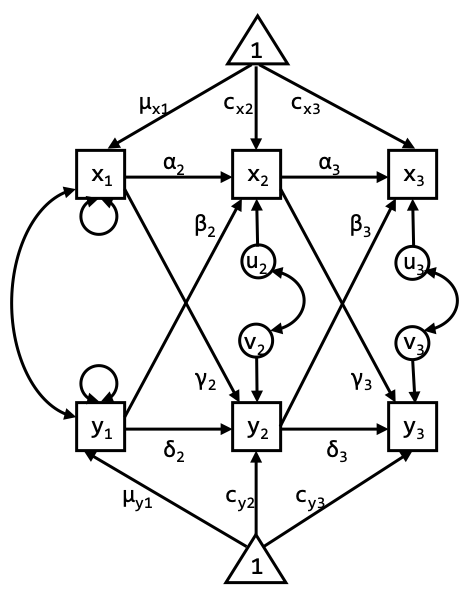
\includegraphics[width=4.16667in,height=\textheight]{CLPM2.png}
\caption{The cross-lagged panel model.}
\end{figure}

Specify the CLPM in Mplus. Regress the observed variables directly on each other over time, as in the graph above. Try to think of where each parameter you estimate should go in the graph.

Click to show answers

The input for this models can be found in \texttt{CLPM.inp}.

\hypertarget{exercise-5}{%
\subsection{Exercise 5}\label{exercise-5}}

Specify the model as in the graph below (the CLPM with centered latent variables), and again include the (significant) parameter estimates in this graph. Tip: do not forget to constrain the measurement error variances of the observed variables to 0.

Click to show answers

The input for this models can be found in \texttt{CLPMalt.inp}.

\begin{figure}
\centering
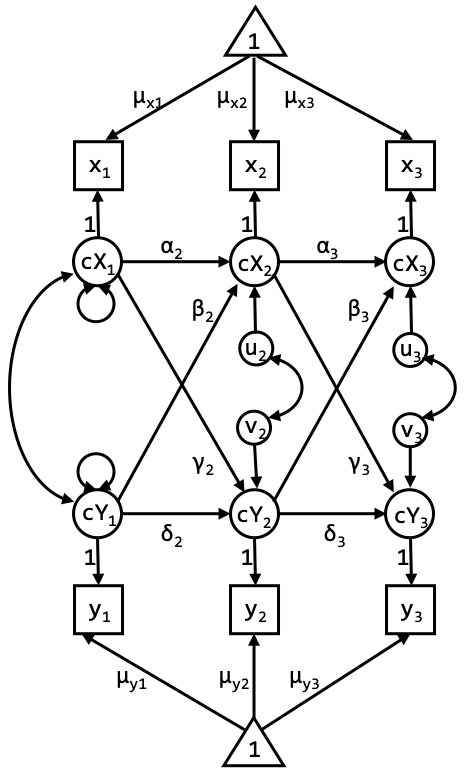
\includegraphics[width=4.16667in,height=\textheight]{CLPM-centered.png}
\caption{The cross-lagged panel model with centered latent variables.}
\end{figure}

\hypertarget{exercise-6}{%
\subsection{Exercise 6}\label{exercise-6}}

The two models should lead to the exact same model fit. Estimate the model and discuss the model fit. When comparing the parameter estimates, what is the difference between the model in question 4 and the model in question 5?

Click to show answers

Model 5 is, just like model 4, a traditional CLPM, but specified in such a way that the mean structure is first separated from the regression part of the model. This implies we model the means, rather than intercepts, which makes it easier to impose the constraint of identical means over time. So, the fit indices and most parameter estimates are equivalent, except for\ldots{} (see next question)

\hypertarget{exercise-7}{%
\subsection{Exercise 7}\label{exercise-7}}

Which parameter estimates differ? How can they be related?

Click to show answers

The difference in parameter estimates is in the means/intercepts. For the first model we estimate the means at wave 1, and intercepts thereafter. For the second model we obtain mean estimates at each wave (although they are referred to as intercepts in the Mplus output).

Again, the reason for this is that in the first model, the means at wave 2 and 3 are partly predicted by the means from previous waves (through the lagged relationships). Therefore, the constants that are estimated should be interpreted as intercepts. In the second model, the mean part (triangles) and the regression part (lagged parameters) are separated.

\hypertarget{exercise-8}{%
\subsection{Exercise 8}\label{exercise-8}}

Constrain the means in the second version of the CLPM. Please do not constrain the mean of \texttt{Dep1}, however, as this constraint proved untenable in exercise 3. Discuss the model fit.

Click to show answers

The input for these models are in \texttt{CLPMalt2.inp}. The chi-square has increased in comparison with the previous model: The reason is that this is a restricted model (a special case of the previous model). We can test whether the increase in misfit is significant using the chi-square difference test: \(\Delta\chi^{2} = 69.59 - 62.98 = 6.61\) with \(\Delta\)\emph{df} = 7 -- 4 = 3, \(p = .0854\). Hence, the constraints are tenable. We can also look at information criteria such as the AIC or BIC. The model with the lowest AIC or BIC is preferred.

\hypertarget{exercise-9}{%
\subsection{Exercise 9}\label{exercise-9}}

Continue with the model from the previous question and constrain all the lagged parameters between wave 1 and 2 to be identical to the lagged parameters between wave 2 and 3. Discuss the model fit, and compare this model to the previous one to see whether the constraint holds.

Click to show answers

The input for these models are in \texttt{CLPMalt3.inp}. The chi-square has again increased in comparison with the previous model: The reason is that this is a restricted model (a special case of the previous model). We can test whether the increase in misfit is significant: \(\Delta\chi^{2} 81.52 - 69.59 = 11.93\), \(\Delta\)(df) = 11 - 7 = 4, \(p = .0178\).

If we stick to an alpha of .05, the constraints must be rejected (as the increase in misfit is significant). Note that we are doing several model comparisons here, so one could also argue that we should use a smaller alpha to guard against an inflated overall type I error. Again, an alternative would be to use information criteria for model comparisons.

\hypertarget{exercise-ri-clpm}{%
\section{Exercise: RI-CLPM}\label{exercise-ri-clpm}}

\hypertarget{exercise-10}{%
\subsection{Exercise 10}\label{exercise-10}}

Specify the RI-CLPM for these data (without any constraints on the lagged parameters over time). Discuss the model fit.

Click to show answers

The input for these models are in \texttt{RICLPM.inp}. This model fits very well; however, it only has 1 \emph{df}, so it is not doing much for data reduction.

\hypertarget{exercise-11}{%
\subsection{Exercise 11}\label{exercise-11}}

Specify the RI-CLPM with the constraints on the grand means at each occasions. Again, please do not constrain the mean of \texttt{Dep1}, however, as this constraint proved untenable in exercise 3.

Click to show answers

The input for these models are in \texttt{RICLPM2.inp}. This model has an acceptable (RMSEA, \(\chi^{2}\)) to good (CFI and TLI) fit. Comparing it to the previous model, we get a chi-square difference test of \(\Delta\chi^{2} = 9.590 - 0.84 = 8.75\), \(\Delta\)\emph{df} = 4 - 1 = 3, \(p = .0328\). This implies that the constraints we impose on the means are untenable (they lead to a significant worsening of model fit). You might therefore decide to ultimately not impose these constraints. However, for didactical reasons, we continue with these constraints in place in the next exercise.

\hypertarget{exercise-12}{%
\subsection{Exercise 12}\label{exercise-12}}

Add the constraints on the lagged parameters to the previous model.

Click to show answers

The input for these models are in \texttt{RICLPM3.inp}. This model fits okay (depending on the measure). Comparing it to the previous model, we get \(\Delta\chi^{2} = 19.74 - 9.59 = 8.15\), \(\Delta\)\emph{df} = 8 - 4 = 4, \(p = .0379\). Again, this implies that constraining the lagged effects to be time-invariant is untenable (it leads to a significant worsening of model fit).

\hypertarget{exercise-13}{%
\subsection{Exercise 13}\label{exercise-13}}

Compare all the models so far simultaneously, using the AIC and BIC. Which model is selected?

Click to show answers

Based on the AIC, the RI-CLPM without any constraints provides the closest fit to the data, followed by the two other RI-CLPMs (and the adjusted means model). Based on the BIC, the RI-CLPM with constraints on the means and the lagged parameters is superior to the other models.

\begin{longtable}[]{@{}lccc@{}}
\toprule
Exercise & Input file & AIC & BIC \\
\midrule
\endhead
1 & Means.inp & 9451 & 9543 \\
3 & Means2.inp & 9442 & 9538 \\
6 & CLPM.inp and CLPMalt.inp & 9494 & 9586 \\
7 & CLPMalt2.inp & 9495 & 9575 \\
8 & CLPMalt3.inp & 9499 & 9563 \\
9 & RICLPM.inp & \textbf{9438} & 9541 \\
10 & RICLPM2.inp & 9441 & 9533 \\
11 & RICLPM3.inp & 9443 & \textbf{9518} \\
\bottomrule
\end{longtable}

\end{document}
